\myparagraph{Purpose}
A very important feature of \textit{Track4Run} is the possibility for an \textit{Organizer} to create a new \textit{Run} defining:
\begin{itemize}
  \item The name of the \textit{Run};
  \item The path of the \textit{Run} through an intercative tool;
  \item The date of the \textit{Run};
  \item The maximum number of participants to the \textit{Run};
  \item The expiration date to enroll in the \textit{Run};
\end{itemize}

\myparagraph{Scenario 1}
Massimo wants to organize a charity \textit{Run} in his little town. He is already registered to \textit{Track4Run} as a Runner. After he has recived all bureaucratic permissions he went to \textit{Track4Run} web site.
With the same credential of the mobile application he logged in the system and in the dashboard he clicked on the "\textit{Create a Run}" button. Massimo set the path through the intercative tool, fixed the date of the \textit{Run} and the missing fields. When everything was completed he clicked on the "\textit{Create}" button and the \textit{Run} went on-line.

\myparagraph{Use Case}
The \textit{Create A Run} use case is analyzed in Table \ref{table:createRunTable}.

\myparagraph{Activity Diagram}
The \textit{Create A Run} activity diagram is shown in Figure \ref{img:createRunActivityDiagram}.

\myparagraph{Mockup}
The \textit{Create A Run} mockup is shown in Figure \ref{img:createRunMockup}.

\myparagraph{Functional requirements}
\begin{enumerate}
  \item The system must not accept a \textit{Run} with date less than or equal to the current one;
  \item The system must not accept a \textit{Run} with expiration date less than or equal to the current one;
  \item The system must not accept a \textit{Run} with maximum number of participants less than or equal to 1.
  \item The system must not accept a \textit{Run} with a path duplication greater or equal to the 50 percent in the same date of an existent one;
  \item The system must let the \textbf{Organizer} leave the creation process at anytime.
\end{enumerate}

\begin{center}
\begin{table}[H]
\begin{tabular}{ | l | p{0.75\linewidth} | }
  \hline
    Actor & \textbf{Organizer} \\ \hline
    Goal & \textbf{[G.10]} \\ \hline
    Input Condition & The \textbf{Organizer} wants to create a new \textit{Run} \\ \hline
    Event Flow & \begin{minipage}[t]{0.7\textwidth}
      \begin{enumerate}
        \item The \textbf{Organizer} opens \textit{Track4Run} service through web application and he/she log in;
        \item The \textbf{Organizer} clicks on the "\textit{Create a Run}" button;
        \item The \textbf{Organizer} inserts path, date, expiration date and maximum number of participants of the \textit{Run};
        \item The \textbf{Organizer} clicks on the "\textit{Create}" button;
      \end{enumerate}
    \smallskip
  \end{minipage} \\ \hline
  Output Condition & The system registers the new \textit{Run} and it notifies the \textbf{Organizer} with a confirmation e-mail. \\ \hline
  Exceptions & \begin{minipage}[t]{0.7\textwidth}
    \begin{itemize}
      \smallskip
      \item If functional requirements 1, 2, or 3 are not satisfied the system notifies the \textbf{Organizer} with an error message and the process goes back to step 3;
      \item In order to prevent functional requirements 4 failure, during the building phase of the path the system continuously checks satisfaction and when the functional requirement is not satisfied it notifies the \textbf{Organizer} with a warning;
      \item If the \textbf{Organizer} decides to leave the creation process this one is aborted.
    \end{itemize}
    \smallskip
  \end{minipage}  \\ \hline
\end{tabular}
\caption{\textit{Create A Run} use case}
\label{table:createRunTable}
\end{table}
\end{center}

\begin{figure}[H]
\begin{center}
  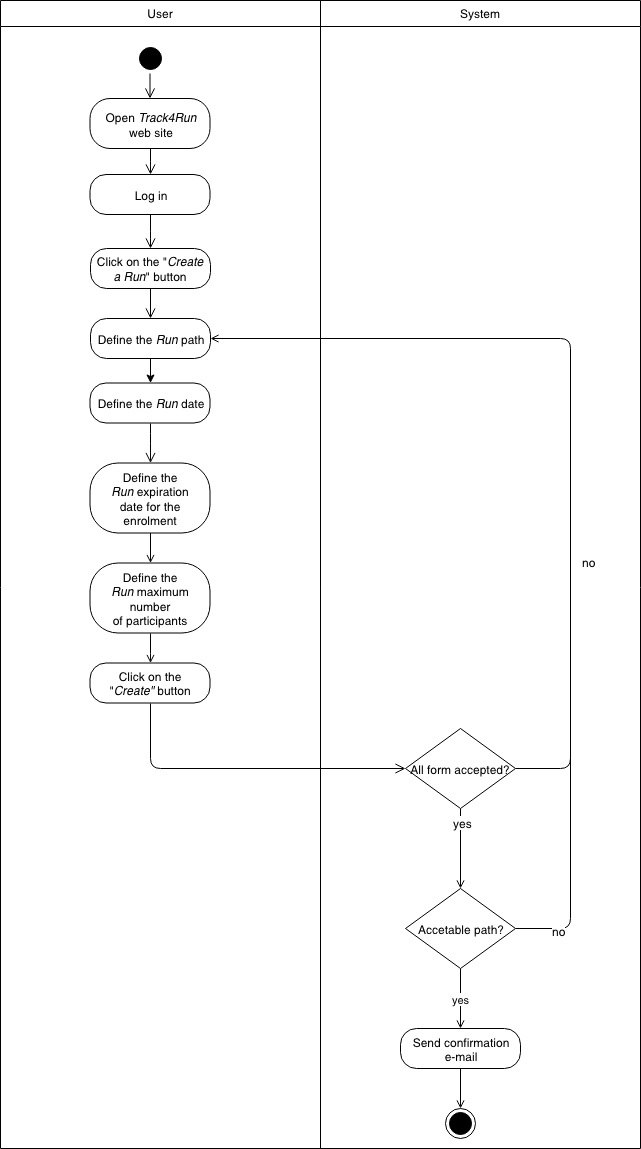
\includegraphics[height=0.6\paperheight]{img/activity/CreateRun.png}
  \hspace{0.05\linewidth}
  \centering
  \caption{\textit{Create A Run} activity diagram from user's point of view}
  \label{img:createRunActivityDiagram}
\end{center}
\end{figure}

\begin{figure}[H]
\begin{center}
  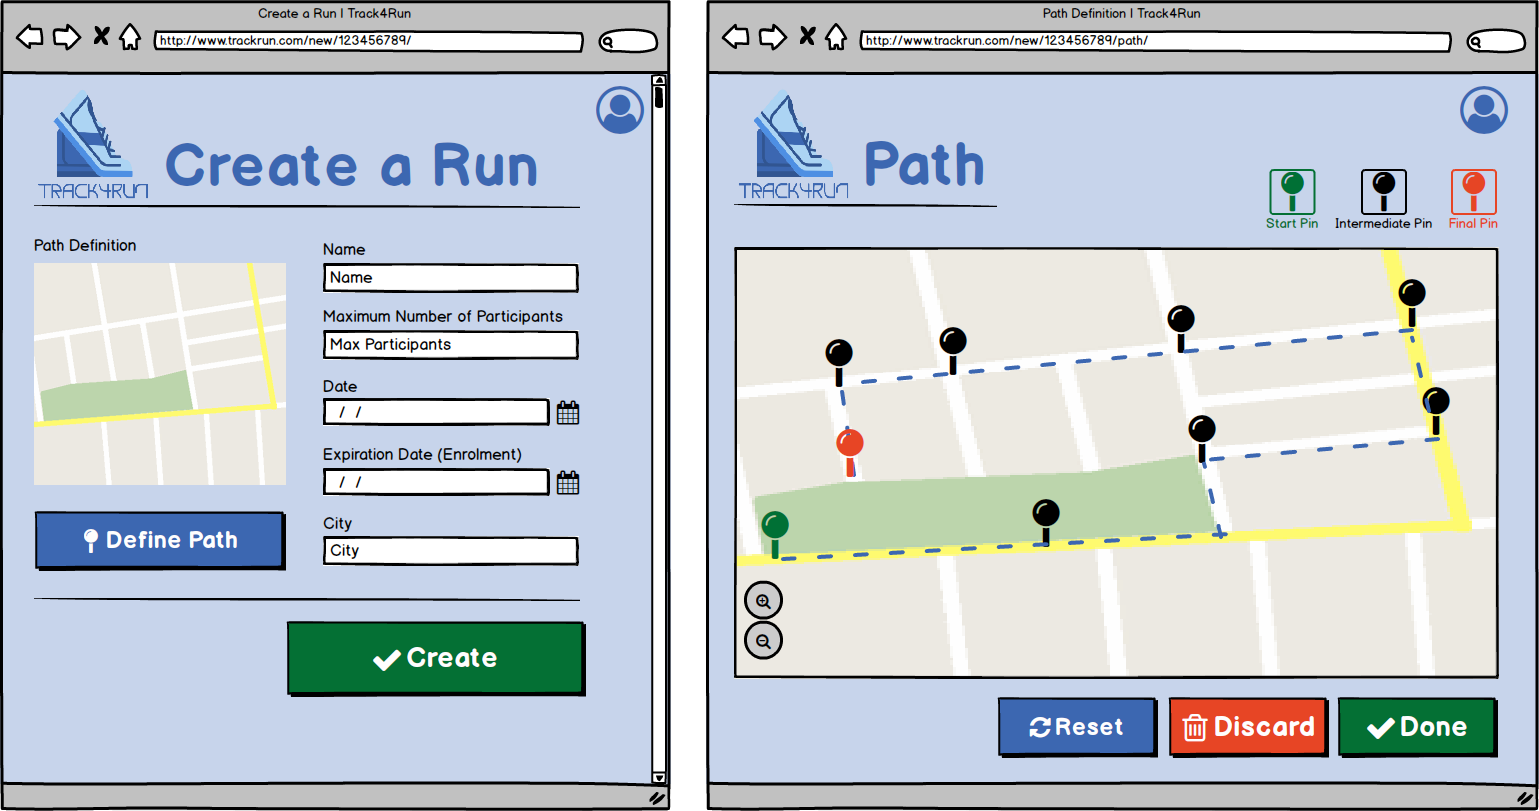
\includegraphics[width=\textwidth]{img/mockup/CreateRun.png}
  \hspace{0.05\linewidth}
  \centering
  \caption{\textit{Create A Run} mockup}
  \label{img:createRunMockup}
\end{center}
\end{figure}
